
\begin{frame}[fragile]{Librería MPAndroidChart en Android}
\textbf{¿Qué es MPAndroidChart?}

\begin{itemize}
    \item Es una librería para la visualización de datos mediante gráficas en Android.
    \item Permite crear gráficos interactivos y altamente personalizables.
\end{itemize}

\vspace{0.3cm}

\textbf{Tipos de gráficas soportadas:}
\begin{itemize}
    \item Gráficas de línea (LineChart)
    \item Barras (BarChart)
    \item Pastel (PieChart)
    \item Dispersión (ScatterChart)
\end{itemize}

\textbf{Ventajas:}
\begin{itemize}
    \item Fácil integración.
    \item Alta personalización (colores, animaciones).
    \item Soporte para interacción (zoom, desplazamiento).
\end{itemize}

\end{frame}



\begin{frame}[fragile]
\frametitle{Demo 15: Graficas con MPAndroid  }
\begin{columns}
\column{0.80\linewidth}

\scriptsize
Del Repositorio Github:
\begin{itemize}
\item Agregar la siguiente linea: \textit{implementation("com.github.PhilJay:MPAndroidChart:v3.1.0")}, al final de la seccion Dependencies del archivo Build.graddle.kts (Module: App).
\item Agregar la siguiente linea: \textit{maven \{ url = uri(``https://jitpack.io'') \}}, al final de la seccion \textit{dependencyResolutionManagement } del archivo settings.graddle.kts.
\item Copiar el archivo \textit{MainActivity\_Demo15.java} (dentro del Folder códigosJAVA) al mismo directorio donde esta el MainActivity.java
\item Copiar el archivo \textit{activity\_main\_demo15.xml} (dentro del Folder Carpeta\_layout) al mismo directorio donde esta el activity\_main.xml
\item Modificar en el archivo \textit{AndroidManifest.xml} la cadena \textit{.MainActivity\_Demo14} por \textit{.MainActivity\_Demo15}.

%\item Ir a la linea 22 de archivo del archivo \textit{MainActivity\_Demo09.java}, poner el cursos en la palabra (en Rojo) \textit{documentfile}, presionar la combinación ALT+ENTER, y seleccionar de la lista desplegable la opcion ``Add dependency on ....''. Esto quitará el error y hara los ajustes necesarios. 
\end{itemize}

%\begin{block}{Demo \#09}
%Un App que permite escribir el contenido de un EditText a un archivo y cargar el contenido de cualquier archivo en el EditText
%\end{block}


\column{0.20\linewidth}

\begin{center}
 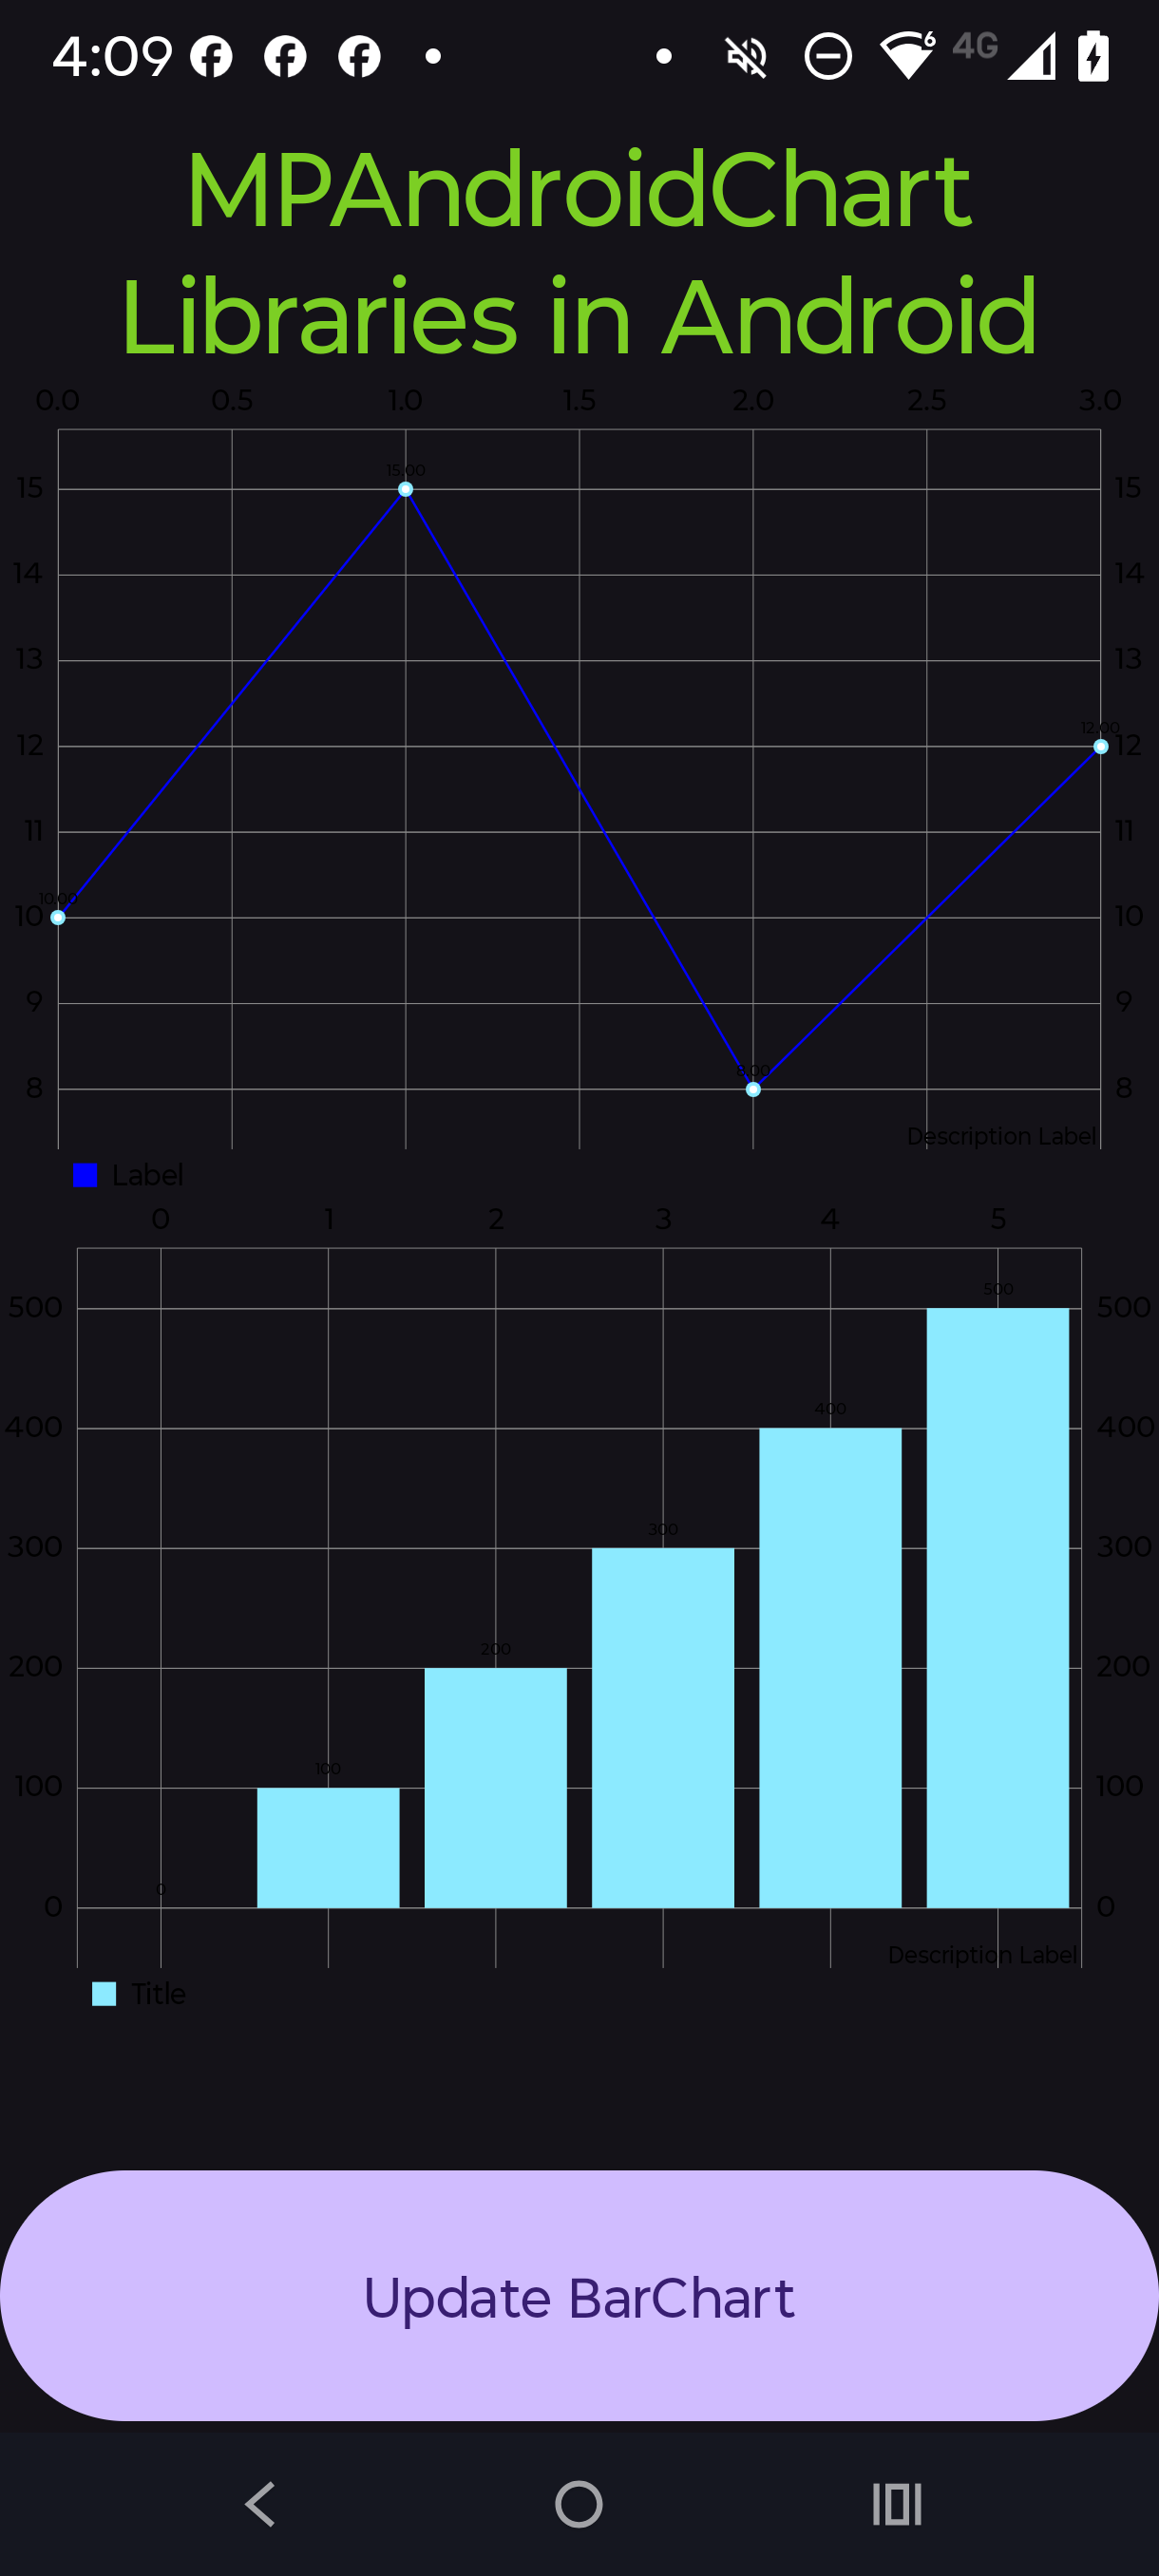
\includegraphics[width=0.98\textwidth]{02_TallerCBTis/figs/Demo15}
\end{center}

\end{columns}

\end{frame}

